\documentclass{article}

\usepackage[final]{style}
\usepackage[utf8]{inputenc} % allow utf-8 input
\usepackage[T1]{fontenc}    % use 8-bit T1 fonts
\usepackage{hyperref}       % hyperlinks
\usepackage{url}            % simple URL typesetting
\usepackage{booktabs}       % professional-quality tables
\usepackage{amsfonts}       % blackboard math symbols
\usepackage{nicefrac}       % compact symbols for 1/2, etc.
\usepackage{microtype}      % microtypography
\usepackage{verbatim}
\usepackage{graphicx}       % for figures
\usepackage{algorithm2e}
\usepackage{commath}
\usepackage{graphicx}


\title{Lecture 5: Q-Learning}

\author{
  Chenglei Si, Goh Yong Liang \\
  sichenglei1125@gmail.com, gyl@u.nus.edu \\
}

\begin{document}

\maketitle


\section{Value Function Learning Theory}
\subsection{Tabular Value Function Learning}
Recall Value-iteration Algorithm:

Loop:

1. Set $Q(s, a) \leftarrow r(s, a) + \gamma E[V(s')]$

2. Set $V(s) \leftarrow \max_{a} Q(s, a)$

To determine if it will converge, we first define the Bellman Backup Operator $B$ as follows:

$BV = \max_a r_a + \gamma T_a V$,

where $r_a$ is the stacked vector of rewards t all states for action $a$, $T_a$ is the matrix of transitions for $a$ such that $T_{a,i,j}=p(s'=i|s=j,a)$.

We always have an optimal policy $V*$ as a fixed point of $B$: 

$V^*(s) = \max_a r(s, a) + \gamma E[V^*(s')]$, so $V^*=BV^*$.

We can prove that value iteration reaches $V^*$ because $B$ is a contraction.

Contraction: for any $V$ and $\overline{V}$, we have $\norm{BV-B\overline{V}}_{\infty} \leq \gamma \norm{V-\overline{V}}_{\infty}$

If we choose $V^*$ as $\overline{V}$, since $BV^*=V^*$, we have: $\norm{BV-V^*}_{\infty} \leq \gamma \norm{V-V^*}_{\infty}$. So it will converge to $V^*$.

Note that:

1. A contraction in a norm is not necessarily a contraction in another norm. 

2. Composition of two contractions in different norms does not necessarily give a contraction.

3. A contraction will give you a fixed point.

\subsection{Non-Tabular Value Function Learning}
Recall fitted value iteration Algorithm:

Loop:

1. Set $y_i \leftarrow \max_{a_i}(r(s_i, a_i)+ \gamma E[V_{\phi}(s_i')])$

2. Set $\phi \leftarrow argmin_{\phi} \frac{1}{2} \sum_i \norm{V'(s) - y_i}^2$

We define a new operator $\Pi$: $\Pi V = argmin_{V' \in \Omega} \frac{1}{2} \sum \norm{V'(s) - V(s)}^2$, $\Pi$ can be interpreted as a projection onto $\Omega$ in terms of L2 norm.

Then we can express fitted value iteration as: 

loop: $V \leftarrow \Pi BV$

While $B$ is a contraction w.r.t. \infty-norm, $\Pi$ is a contraction w.r.t. L2-norm, $\Pi B$ is not a ontraction of any kind. Hence, fitted value iteration does not converge.

Similar proof can be done for fitted Q iteration algorithm as well:

Recall fitted Q iteration Algorithm:

Loop:

1. Set $y_i \leftarrow r(s_i, a_i) + \gamma E[V_{\phi}(s_i')]$

2. Set $\phi \leftarrow argmin_{\phi} \frac{1}{2} \sum_i \norm{Q_{\phi}(s_i, a_i) - y_i}^2$

We define $B$ and $\Pi$ slightly differently here: 

$B$: $BQ = r + \gamma T \max_a Q$

$\Pi$: $\Pi Q = argmin_{Q' \in \Omega} \frac{1}{2} \sum_i \norm{Q'(s,a) - Q(s,a)}^2$

Then fitted Q-iteration is: loop: $Q \leftarrow \Pi BQ$. $\Pi B$ is not a contraction of any kind, so it does not converge. The same applies to online Q-learning as well.


\section{How to make Q-learning work}
\subsection{Problem 1: Correlated samples in online Q-learning}
There are 2 main problems with online Q-iteration: 
1. Sequential states are strongly correlated (and we don't want samples to be correlated). 2. Target value is always changing.

Solution 1: synchronized/asynchronous parallel Q-learning

Solution 2: Replay Buffers

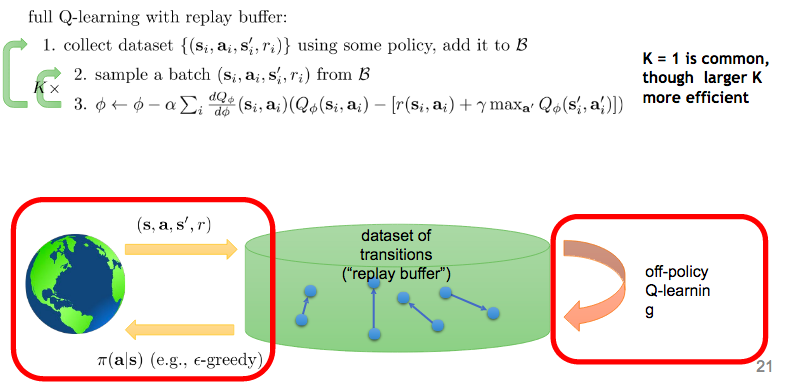
\includegraphics[scale=0.5]{replayBuffer.png}

\subsection{Problem 2: Moving Target in Regression}
Q-learning is not exactly gradient descent because the target $y$ depends on Q itself. In other words, the target keeps changing,

Solution: Q-learning with target networks

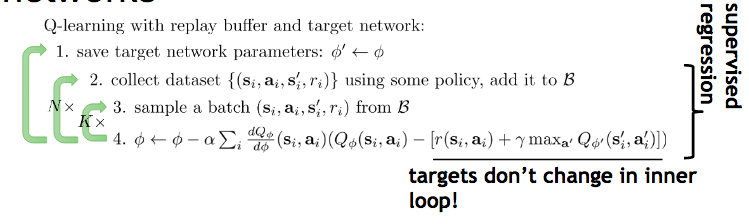
\includegraphics[scale=0.5]{targetNet.png}

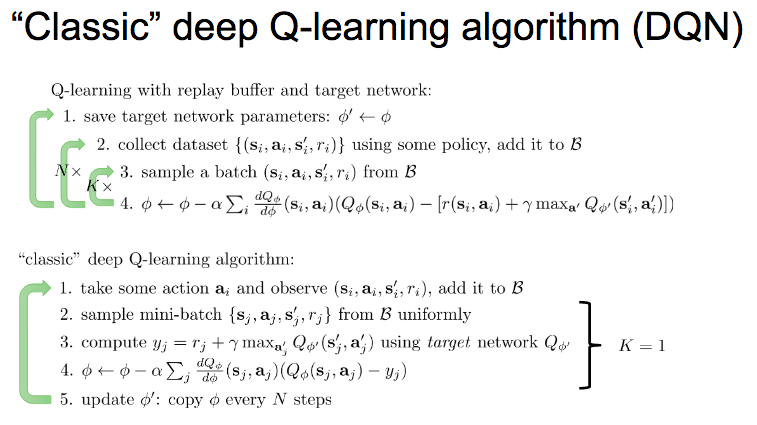
\includegraphics[scale=0.5]{DQN.png}

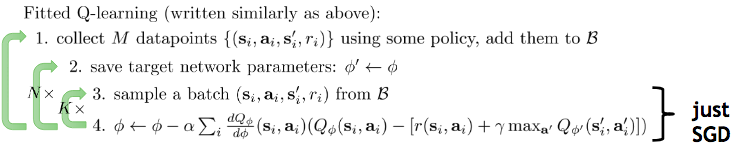
\includegraphics[scale=0.5]{FQL.png}

\textbf{Other Solutions:}

1. Prioritized Experience Replay:

Weight sampling from replay buffer by TD-error: $\delta_t = r_{t+1} + \gamma V(s_{t+1}) - V(s_t)$, Correct for introduced bias via importance-sampling weights.

2. Hindsight Experience Replay:

Consider bit-flipping environment:

State space: S in \{0, 1\}$^n$
  Action space: A = \{0, 1, ..., n-1 \}

Each episode is a uniformly sampled initial state, and target state, and the reward is -1 if not in the target state.

\subsection{Problem 3: Overestimation in Q-learning}
For random variables $X_1, X_2$:
$E[max(X_1, X_2)] \geq \max(E[X_1], E[X_2])$.

In target value $y_j = r_j + \gamma \max_{a_j'} Q_{\phi'}(s_j', a_j')$, $\max_{a_j'} Q_{\phi'}(s_j', a_j')$ overestimates the next value. Note that $\max_{a_j'} Q_{\phi'}(s_j', a_j')= Q_{\phi'}(s', argmax_{a'}Q_{\phi'}(s', a'))$ here both the value and action come from $Q_{\phi'}$. We want the noise to be decorrelated. 

Solution: Double Q-Learning

Idea: Don't use the same network to to choose the action and evaluate value. In practice, just use the current and target network:

$y \leftarrow r+ \gamma Q_{\phi'}(s', argmax_{a'}Q_{\phi}(s', a'))$



\section{Q-Learning with continuous actions}
In target value $y_j = r_j + \gamma \max_{a_j'} Q_{\phi'}(s_j', a_j')$, how do we perform the max?

\subsection{Option 1: Optimization}
Gradient based optimization (e.g., SGD) a bit slow in the inner loop.
Simple Solution:

$max_a Q(s, a) \approx \max\{ Q(s,a_1), ..., Q(s, a_N)\}$

More accurate solutions: Cross-Entropy Method, Covariance Matrix Adaptation Evolution Strategy

\subsection{Option 2: Easily maximizable Q-functions}
Use function class that is easy to optimize:

Normalized Advantage Functions. NAF represents the critic by a quadratic function with a negative curvature:

$Q_{\phi}(s, a) = -\frac{1}{2} (a- \mu_{\phi}(s))^T P_{\phi}(s)(a- \mu_{\phi}(s)) + V_{\phi}(s)$

argmax$_a Q_{\phi} (s, a) = \mu_{\phi}(s)$

$\max_a Q_{\phi} (s, a) = V_{\phi} (s)$

\subsection{Option 3: learn an approximate maximizer}
Basic idea: Train Neural Networks that approximates max function given state and possible actions.

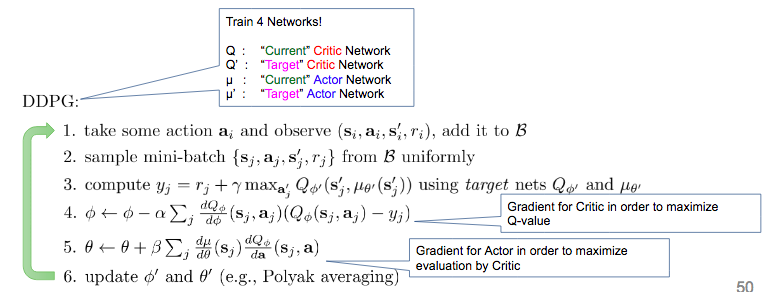
\includegraphics[scale=0.5]{DDPG.png}

\subsection{Practical Tips}
1. Q-learning takes some care to stabilize
Test on easy, reliable tasks first, make sure your implementation is correct.

2. Large replay buffers help improve stability

3. It takes time, be patient – might be no better than random for a while.

4. Start with high exploration (epsilon) and gradually reduce.

5. Bellman error gradients can be exploded; clip gradients, or use Huber loss
Huber loss is robust against outlier compared to squared loss

6. Double Q-learning helps a lot in practice, simple and no downsides.

7. N-step returns also help a lot, but have some downsides.

8. Schedule exploration (high to low) and learning rates (high to low),  Adam optimizer can help too.

9. Run multiple random seeds, it’s very inconsistent between runs.




























% References
\small
\bibliographystyle{plain}
\bibliography{bibliography}
On Improving Deep Q-Learning: DDQN, Prioritized Experience Replay, Fixed Q-targets:

https://medium.freecodecamp.org/improvements-in-deep-q-learning-dueling-double-dqn-prioritized-experience-replay-and-fixed-58b130cc5682


Prioritized experience replay: 

https://web.stanford.edu/class/psych209/Readings/MnihEtAlHassibis15NatureControlDeepRL.pdf 

https://arxiv.org/pdf/1511.05952.pdf 

https://becominghuman.ai/learning-from-mistakes-with-hindsight-experience-replay-547fce2b3305
\end{document}
